\documentclass[serif,9pt]{beamer}
\usetheme{tree}
%\usepackage{german}
\usepackage[latin1]{inputenc}
\usepackage[spanish]{babel}

% Images
\usepackage{graphicx}
\usepackage{subfigure} % subfiguras
\usepackage{caption}
\usepackage{float}
\captionsetup[table]{labelformat=empty}
\captionsetup[figure]{labelformat=empty}

\usepackage{amsmath}

\usepackage{listings}
\lstset
{ %Formatting for code in appendix
  language=C++, % choose the language of the code
  basicstyle=\fontfamily{pcr}\selectfont\footnotesize\color{black},
  keywordstyle=\color{darkorange}\bfseries, % style for keywords
  numbers=left, % where to put the line-numbers
  numberstyle=\tiny, % the size of the fonts that are used for the line-numbers     
  backgroundcolor=\color{white},
  showspaces=false, % show spaces adding particular underscores
  showstringspaces=false, % underline spaces within strings
  showtabs=false, % show tabs within strings adding particular underscores
  tabsize=2, % sets default tabsize to 2 spaces
  captionpos=b, % sets the caption-position to bottom
  breaklines=false, % sets automatic line breaking
  breakatwhitespace=false, 
}

\AtBeginSection[]
{
  \begin{frame}<beamer>{Contenido}
    \tableofcontents[currentsection]
  \end{frame}
}

\definecolor{darkorange}{rgb}{0.94,0.4,0.0}

\begin{document}
\setbeamertemplate{navigation symbols}{}

\title{Pr�ctica 4: Algoritmos Backtracking}  
\author{David Cabezas Berrido}
\date{}

\begin{frame}
\titlepage
\end{frame}

\begin{frame}\frametitle{�ndice}\tableofcontents
\end{frame}

\section{Introducci�n}
\begin{frame}\frametitle{Introducci�n}
Se celebra una cena de gala con $n$ invitados, cada invitado tendr�
sentados a dos comensales a su izquierda y a su derecha y conocemos la
afinidad que tiene cada invitado $i$ con cada invitado $j$. El nivel
de conveniencia total de una asignaci�n es la suma de las afinidades
de cada invitado con las personas de su izquierda y derecha, Debemos
maximizar este valor.
\end{frame}

\section{Algoritmo}

\subsection{Fuerza Bruta}

\begin{frame}
  \begin{center}
    \Huge Algoritmo de fuerza bruta
  \end{center}
\end{frame}

\begin{frame}[fragile]\frametitle{Fuerza Bruta}
\begin{lstlisting}
void bruteForce(const Cena& cena, const vector<int> &sentados,
     vector<int> &bestSol, int currentAffinity, int& bestAffinity)
   {
     if(sentados.size() == cena.getN()){
       currentAffinity += cena.getAfinidad(sentados.back(),sentados.front())
       + cena.getAfinidad(sentados.front(),sentados.back());
       if(currentAffinity > bestAffinity){
         bestAffinity = currentAffinity;
         bestSol = sentados;
       }
       return;
     }
     
     int aff;
     vector<int> aux;
     
     for(int i = 1; i < cena.getN(); i++){
       aff = currentAffinity;
       aux = sentados;
       if(find(sentados.begin(),sentados.end(),i)==sentados.end()){
         aux.push_back(i);
         aff += cena.getAfinidad(i,sentados.back())
         + cena.getAfinidad(sentados.back(),i);
         backtracking(cena, aux, bestSol, aff, bestAffinity);
       }
     }
   }
\end{lstlisting}
\end{frame}

\subsection{Backtracking}

\begin{frame}
  \begin{center}
    \Huge T�cnica de Backtracking
  \end{center}
\end{frame}

\begin{frame}[fragile]\frametitle{C�digo}
\begin{lstlisting}
  int cotaAfinidad(const vector<int> &sentados, int afActual) const{
    int maxA = afActual;
    int max1, max2;

    for(int i = 1; i < n; i++)
      if(find(sentados.begin(),sentados.end(),i)==sentados.end()){
        mayoresAfinidades(i,max1,max2);
        maxA += max1+max2; 
      }
   
    mayoresAfinidades(sentados.front(),max1,max2);
    maxA += max1;
    mayoresAfinidades(sentados.back(),max1,max2);
    maxA += max1;

    return maxA;
  }
\end{lstlisting}

En la l�nea 13 de la funci�n anterior:

\begin{lstlisting}
    if(cena.cotaAfinidad(sentados, currentAffinity) <= bestAffinity){
      return;
    }
\end{lstlisting}
\end{frame}

\section{Resultados emp�ricos}

\begin{frame}{Tiempos de ejecuci�n obtenidos}
  \begin{figure}[!hbp]
  \centering
  \label{tab:tiempos}
  \begin{tabular}{| c | c | c | c |}
    \hline
    \multicolumn{1}{|c|}{$\textbf{n}$}& \textbf{Backtracking}&
    \textbf{Fuerza Bruta}& \textbf{Ganancia} \\ \hline
     3 & 1.81e-05  & 2.28e-05  & 1.259669  \\ 
     4 & 6.68e-05  & 1.49e-05  & 0.223054  \\ 
     5 & 7.02e-05  & 6.38e-05  & 0.908832  \\ 
     6 & 0.0003676 & 0.0003573 & 0.971980  \\ 
     7 & 0.0017335 & 0.0020342 & 1.173464  \\ 
     8 & 0.0070328 & 0.014561  & 2.070441  \\ 
     9 & 0.028686  & 0.128955  & 4.495398  \\ 
    10 & 0.170039  & 1.27693   & 7.509630  \\ 
    11 & 0.950164  & 13.8355   & 14.561170 \\ 
    12 & 2.99369   & 165.75    & 55.366454 \\ \hline
  \end{tabular}
\end{figure}
\end{frame}

\begin{frame}{Gr�fica tiempos backtracking}
  \begin{figure}[H]
  \centering
  \subfigure[Algoritmo Backtracking]{\label{graf:backtracking}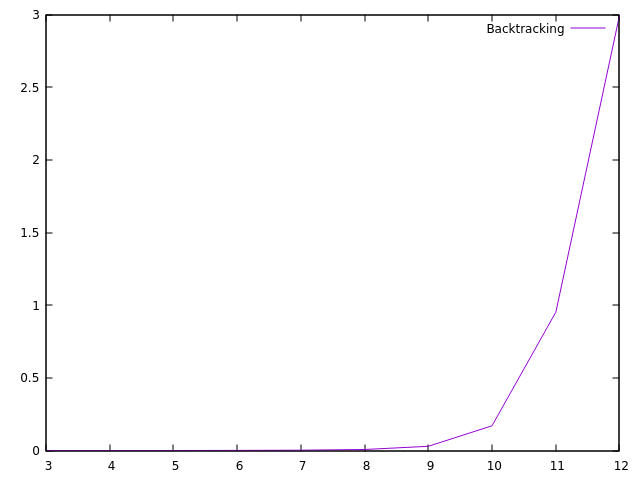
\includegraphics[width=100mm]{graficas/backtracking}}
  \end{figure}
\end{frame}

\begin{frame}{Gr�fica comparativa con fuerza bruta}
  \begin{figure}[H]
  \centering
  \subfigure[Comparaci�n con algoritmo de fuerza bruta]{\label{graf:comparacion}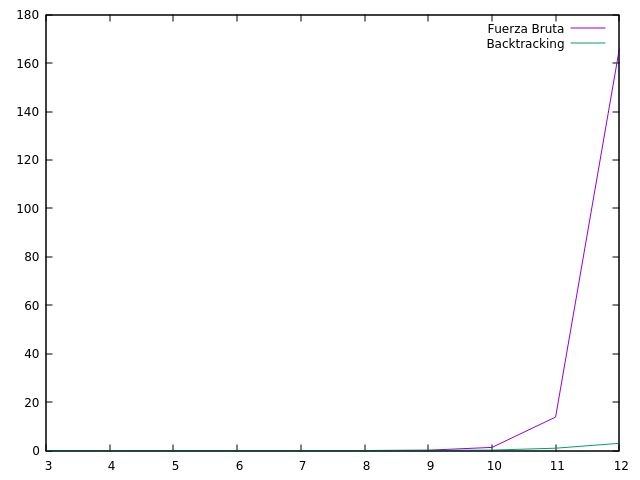
\includegraphics[width=100mm]{graficas/comparacion}}
  \end{figure}
\end{frame}

\end{document}